\documentclass{sig-alternate}
% \documentclass{acm_proc_article-sp}
\usepackage{graphicx}
\usepackage{hyperref}

\usepackage{subfig}
%\usepackage{caption}
\DeclareCaptionType{copyrightbox}
%\usepackage{subcaption}

\usepackage{verbatim}
\makeatletter
\newif\if@restonecol
\makeatother
\let\algorithm\relax
\let\endalgorithm\relax
\usepackage[linesnumbered]{algorithm2e}

\makeatletter
\newcommand{\nosemic}{\renewcommand{\@endalgocfline}{\relax}}% Drop semi-colon ;
\newcommand{\dosemic}{\renewcommand{\@endalgocfline}{\algocf@endline}}% Reinstate semi-colon ;
\newcommand{\pushline}{\Indp}% Indent
\newcommand{\popline}{\Indm\dosemic}% Undent
\makeatother

\pdfinfo{
   /Title  (acm-mm13-short)
}

\begin{document}

\title{From Digital Photographs to Digital Stories}

\numberofauthors{2}
\author{
\alignauthor
Person 1\\
       \affaddr{University}\\
       \email{email}\\
\alignauthor
Person 2\\
       \affaddr{University}\\
       \email{email}\\
}


\maketitle
\begin{abstract}
Personal photographs witness events/subevents in our lives. Oftentimes, a sequence of these events represents narrative stories with characters (i.e., participants), and spatiotemporal settings. Storytelling is a simple way of sharing and communicating life experiences with other people. In this paper, we present an automated technique to evoke the finest subevents from the photo stream of an event - using image metadata (timestamp, location, and camera parameters), information about the user, ontological event model, mobile device connectivity, web services, and external data sources – to build digital stories around those events. We describe Event Ontology Augmentation that is a new technique to infer, refine, and validate expressive event tags in the context of digital storytelling. In this technique, an ontological event model (containing event/entity classes and relationships) is used to describe the vocabulary for a general story domain like ‘trip’. The domain event-ontology is extended with context-information from heterogeneous data sources using abductive reasoning. We introduce ‘plausibility measure’ for ranking and selecting the best possible subevent category related to a group of photos in a photo stream. In addition, we propose a new agglomerative clustering method for partitioning photos, which uses timestamp, location, and camera parameters in the EXIF header of the input photos. 
\end{abstract}

\category{H.3.3}{Information Search and Retrieval}{Information Filtering}
\category{H.3.4}{Systems and Software}{Information Networks}
\category{H.5.1}{Multimedia Information Systems}{} 

\terms{Design, Algorithms, Experimentation}
\keywords{CueNet, context, discovery, event, personal, photo, tagging}

\section{Introduction}
Intro

\section{Context}
Some context about context.

\section{Progressive Discovery}
Blah \cite{westermann2007toward, gupta2011managing}



\begin{figure}[t]
\centering
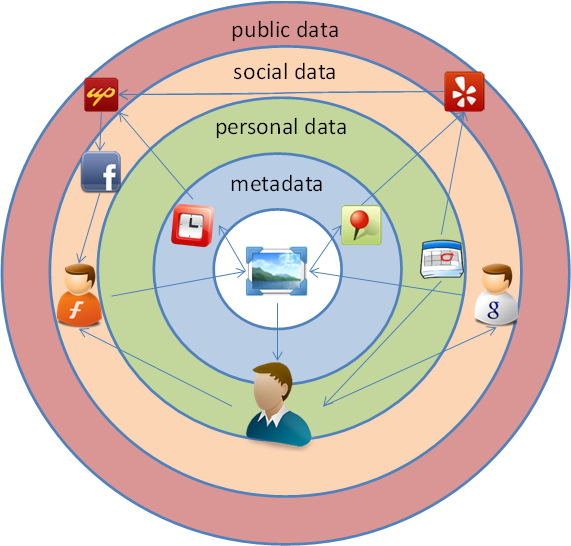
\includegraphics[width=0.48\textwidth]{media/prog-discovery.png}
\caption{Example of Progressive Discover.}
\label{fig:cuenet-arch}
\end{figure}

\bibliographystyle{abbrv}
\bibliography{sigproc}
\end{document}
